\documentclass[10pt, conference]{IEEEtran}

% \usepackage{hyperref}	%To get rid of EDAS warning: External links are not allowed
\usepackage{amsmath}
%\pdfpagewidth=8.5in
%\pdfpageheight=11in
\usepackage{graphicx}
\usepackage{array}                 % nicer looking arrays?
\usepackage{cite}
\usepackage{url}
\usepackage{multirow} 		% multiple rows in a table
%\usepackage{subfigure}
\usepackage{subfig}
\usepackage{color,latexsym,amsfonts,amssymb}
\usepackage{bm} %use \bm instead of \mathbf

\makeatletter
\def\ps@headings{%
\def\@oddhead{\mbox{}\scriptsize\rightmark \hfil \thepage}%
\def\@evenhead{\scriptsize\thepage \hfil \leftmark\mbox{}}%
\def\@oddfoot{}%
\def\@evenfoot{}}
\addtolength\textfloatsep{-3ex}

\title{Energy-Efficient Sleeping in Wireless Sensor Networks}

%%%%% AUTHORS %%%%%
\author{\IEEEauthorblockN{Deepak Jha \texttt{deepakjha@cs.ucsb.edu}}
\IEEEauthorblockN{Kai Howelmeyer \texttt{hoewelmeyer@umail.ucsb.edu}}
\IEEEauthorblockN{Faisal Nawab \texttt{nawab@cs.ucsb.edu}}
\vspace{5pt}
\IEEEauthorblockA{University of California, Santa Barbara\\
Department of Computer Science
}}

\begin{document}

\maketitle

\begin{abstract}
	This paper explores a simple network topology in wireless sensor networks (WSN). Three endnodes connected to a coordinator. Each endnode is connected to a battery. In order to maximize network longetivity, the sleeping time of each of the endnodes is maximized while the delay for the response time is limited. This paper contributes a model describing the connection between sleeping duration, workload, and delay in a given topology. The model is evaluated on a hardware testbed as well as in simulations.
\end{abstract}

\begin{keywords}
	Wireless Sensor Networks (WSN), Energy Efficiency, ZigBee, Sleeping, Polling.
\end{keywords}

\section{Introduction}\label{sec:Intro}

Wireless Sensor Networks (WSNs) use sensors to measure a wide variety of live data and actuators to manipulate their environments. Data are communicated between nodes and sinks. WSNs are self-configuring, inherently small, low-cost, and low-power. This makes it a suitable technology for use in monitoring and tracking applications. Many of the envisioned applications of sensor networks require a large-scale deployment that comprises thousands of sensor nodes, e.g., the Internet of things \cite{22} and sensor database systems \cite{2}. With a large number of sensor nodes, it becomes challenging to maintain all collected data in a centralized unit (or multiple centralized units). Moreover, the demand for data might vary from node to node. Keeping the node awake at all times is a waste of communication resources and will ultimately drain the nodes power prematurely. A energy-aware demand-driven transactional protocol is needed to mitigate this waste of resources. Many papers propose a distributed approach to data-management in sensor networks \cite{2,4.11,23}. Instead of having a central database collecting sensor readings from individual nodes, the data is stored and distributed over the nodes themselves. Queries then extract the necessary data from the sensor nodes. 

In a transactional distributed scheme the node needs to be alerted for any data queries. Thus, making the node awake (i.e., consuming energy) even if it is not sending or collecting data. A desirable property of WSNs is power-efficiency. The main objective of this work is to save power and prolong the life of nodes by making them consume as less power as possible. Having low sleep times will make a node handle incoming requests faster, since they are only waiting for a short period. However, a longer sleeping period will minimize the number of switches between sleeping and active modes. These switches incur a communication overhead; a newly awaken node must poll its parent node for requests. Furthermore, the waking time (the time required for a node to switch from sleeping to active) ranges between 2 to 13.2 milliseconds for XBEE series 2 nodes \cite{19}. Thus, we aim to maximize sleeping time while we maintain QoS requirements.

The paper is divided as follows. Section 2 details the motivation of our research, Section 3 outlines related work, Section 4 summarizes the technical background of the prototype, Section 5 describes the system design of the prototype, Section 6 proposes a model for QoS in our system, Section 7 evaluates the model both with the prototype and with simulations, Section 8 concludes.

\section{Motivation} \label{sec:motivation}

%/* Write about the battery drain experiment and how a longer battery life can be achieved by having a longer sleep resp. poll time.*/

\begin{figure}[t]
\centering
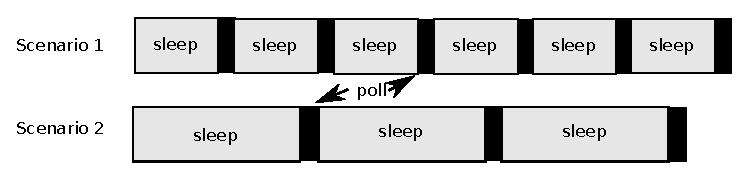
\includegraphics[scale=0.65]{figures/drawing.eps}
\caption{A motivating scenario on the effect of sleep cycle time on energy consumption}
\label{fig:motivating}
\end{figure}

In our project we tackle one of the main challenges in WSNs, namely energy inefficiency. Sensors have a limited amount of power. In the absence of any tasks, a node wastes its energy waiting for transmissions. Making a node sleep (i.e., consume less power) in inactive periods is a well-studied way to leverage unwanted use of power \cite{1}. However, we consider the effect of the sleep cycle duration on energy consumption. We show a motivating example in Figure~\ref{fig:motivating}. In it we consider two scenarios where no data exist to be received. The first scenario have a sleep cycle duration of half the second scenario. The black rectangles denote the period of polling for buffered packets. It is apparent that scenario one consumes more energy since it is switching to poll for received packets more often. The effect of sleep cycle duration extends to scenarios with active receptions and can be intuitively derived.  

Given our motivation, the main objective of our work is to maximize sleeping times. However, there is a tradeoff between sleep times and QoS requirements (we consider delay); longer sleep cycle duration translate to larger delay times. A query-based framework is considered for our implementation \cite{2}. We will use ZigBee and IEEE 802.15.4 \cite{3} as our system's infrastructure. The objective of our work is three-fold: First, we will deploy a query-based WSN using Arduino microcontrollers \cite{17} and XBEE modules \cite{18}. Second, we will implement the query-based scheme over QualNet simulator~\cite{16}. Using the deployment and simulation framework we can study the system for the effects of sleep cycle duration on QoS and energy consumption. Third, a mathematical model will be constructed to capture QoS and energy characteristics. From the model, a formula for determining maximum sleeping times is derived. The resulted formula will be tested in the deployment (as a proof-of-concept prototype) and in simulation (to investigate scalability).

The main contribution of our work is to produce a mathematical model that can be used to capture QoS with respect to sleep behavior in WSNs. This model can then be used to derive suitable sleeping times when given certain QoS characteristics and network load. A queueing system \cite{21} can be used to model this problem. An M/G/1 queueing model with vacations \cite{20} is, we claim, suitable for such a problem.

Another challenge is to deploy and simulate a query-based WSN. A full deployment of transaction handling distributively in WSNs would include transaction processing and optimization, routing, aggregation, etc. \cite{2}. We will start with a simple query-based scheme in our deployments. However, we will design it so it would be possible to incrementally develop it to include more transactional features. 


\section{Related Work} \label{sec:relwork}

\section{Background}\label{sec:background}

\begin{figure}[t]
\centering
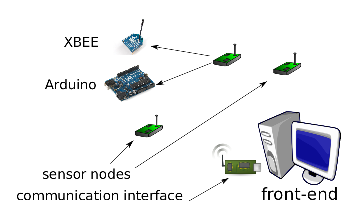
\includegraphics[scale=1.2]{figures/topology.eps}
\caption{Components used in the prototype}
\label{fig:topology}
\end{figure}

%/* speak here about arduino, XBee, ZigBee protocol, and 802.15.4 */
A depiction of our prototype is supplied in Figure~\ref{fig:topology}. It consists of a front-end that receives external requests and delivers readings for outside users. The back-end is a collection of sensor nodes consisting of a micro-controller and a wireless module. A detailed description of used components follows:
\begin{itemize}
\item{\emph{Arduino}: Arduino is a micro-controller capable of sensing the environment by receiving input from sensors in its surroundings. The micro-controller on the board is programmed using the Arduino programming language (based on C/C++ library) and the Arduino development environment (based on \textit{Processing}). In Arduino the connectors are exposed in such a way that allows CPU boards to be connected to a variety of interchangeable add-on modules. In our experiments we use Arduino Uno boards.}
\item{\emph{XBEE}: XBee is a radio module based on IEEE 802.15.4 networking protocol providing wireless end-point connectivity to devices.  It is designed for high-throughput applications which require low latency and predictable communication timing. AT commands are used to control the radio settings. They can operate either in a transparent data mode or in a packet based (API) mode. In the transparent mode data coming into the DIN (Data IN) pin gets directly transmitted to the intended receiving radios without any modification. Incoming packets can either be directly addressed to one target or broadcast to multiple targets. This mode is primarily used in instances where an existing protocol cannot tolerate changes to the data format. We use XBee series 2 modules.}
\item{\emph{ZigBee}: ZigBee is a specification for a suite of high level communication protocols using small, low-power digital radios based on an IEEE 802 standard for Personal Area Network (PAN). ZigBee builds upon the physical layer and medium access control defined in IEEE standard 802.15.4 (2003 version) for low-rate wireless PANs.  It is targeted at radio-frequency (RF) applications that require a low data rate, long battery life, and secure networking. ZigBee data rate varies from 20 kbps to 900 kbps but 250 kbps is best suited for periodic or intermittent data or a single signal transmission from a sensor or input device. The current ZigBee protocol supports beacon and non-beacon enabled networks. In our experiments we operate in non-beacon mode. There are three different types of Zigbee devices: 
\begin{itemize}
\item{\emph{ZigBee Coordinator (ZC)}: it forms the root of the network tree and might bridge to other networks. There is exactly one ZC per network. }
\item{\emph{ZigBee Router (ZR)}: it can run an application and can also act as an intermediate router. }
\item{\emph{ZigBee End Device (ZED)}: It has the capability to talk to the parent node. It cannot relay data from other devices. This relationship allows the node to be asleep a significant amount of the time thereby giving long battery life.}
\end{itemize}
}
\end{itemize}


\section{System design}\label{sec:design}

\subsection{WSN as a DB}
\subsection{Sleeping Scheme}
/* what do we understand under sleeping and how did we implement it? */


\subsection{Front-end design}
/* This subsection on the front-end (server) that will take queries and process them and transform them to light-weight queries sent to the sensors */

\subsubsection{Query processing}
/* The process of breaking the query to simpler light-weight queries. How data is assembled from nodes etc */

\subsubsection{Concurrency gurantees}
/* I was thinking that we should add actuators to our system. For example, a sensor to detect if the light is on and is capable of turning the light on/off (or something like, if the temperature is above 25 deg. turn AC on). What is here is how to gurantee that a query is right. I propose to treat it as timestamp-based concurrency management, and the proof of correctness is available. Also, we should talk that a property of this scheme is that a correct behavior is maintained while that we always accept read requests, but a write can be rejected.
BTW, I beleive this is VEEEERY novel, they usually talk about sensing only.
 */

\subsection{Back-end design}

\subsection{Hardware}
We are using three Arduino Uno microcontrollers as end nodes in our prototype topology. Each of these microcontrollers is connected to a XBee Series 2 module for wireless communication. A fourth XBee module is directly connected to a computer and acts as the coordinator of the network.

\subsection{Software}
The host connected to the XBee controller is running a LAMP-stack, i.e. a linux machine equipped with apache, MySQL, and PHP.
/* elaborate here */


 

\section{Modeling wait time}\label{sec:model}

In this section, we will develop a model of delay and queue utilization of our system. The Round Trip Time (RTT) experienced by each packet is described by the following sum:
\begin{equation}
\psi = W + W_{end node}
\end{equation}
where $W$ is the wait time in the front-end, $W_{end node}$ is the wait time experienced by the end-node. We focus on the $W$ since it is effected by the dynamics of sleeping and buffering, where $W_{end node}$ is predictable and can be substituted with a constant value dependent on the channel characteristics and processing requirements. We will use an M/G/1 queue model with vacations. We denote the amount of incoming traffic to the network by $\lambda$. The distribution of inter-arrival times, $A(t)$, is exponential, where the mean is $\frac{1}{\lambda}$. The service time, denoted as $X$, is translated as the time required to service the packet in the head of the queue of the front-end. This value is dependent on the contention of the medium.

%We start by observing the waiting time. It is the summation of time spent in the queue in addition to the service time, given by
%\begin{equation}
%W = R + \sum_{j \in queue} X_j
%\end{equation}
%where $R$ is the residual service time seen by an arriving query and $X_j$ is the service time for query $j$. Taking expectations we have
%\begin{equation}
%W = R + \bar{X}N_q
%\end{equation}
%where $N_q$ is the average queue utilization. Using Little's Formula~\cite{21} we arrive to the following
%\begin{equation}
%\label{eq:waiting}
%W = \frac{R}{1 - \rho}
%\end{equation}
%where $\rho$ is the traffic intensity equal to $\lambda\bar{X}$. Thus, we need to find an expression for the average residual time seen by an incoming query. This can be obtained by calculating the average of residual times in a time interval $[0, t]$
%\begin{equation}
%\frac{1}{t} \int_0^t r(\tau) d\tau
%\end{equation}
%where $r(\tau)$ is the residual time at time $\tau$. The integral is the summation of the contribution of each service time in the considered time interval. The contribution of each service time is half the square of that query's service time. The same is applied to vacations, where the contribution of each vacation period is half the square of that query's service time. This is demonstrated as the following:
%\begin{equation}
%\frac{1}{t} \int_0^t r(\tau) d\tau = \frac{1}{t} \sum_{i \in S(0,t)} \frac{X_i^2}{2} + \frac{1}{t} \sum_{i \in V(0,t)} \frac{V_i^2}{2}
%\end{equation}
%where $S(0,t)$ and $V(0,t)$ are the set of serviced queries and vacations in the time period $[0, t]$, respectively, and $V_i$ is the vacation time. Solving the summation and taking the limit of $t$ approaching infinity we obtain
%\begin{equation}
%\label{eq:residual}
%R = \frac{\lambda\bar{X^2}}{2} + \frac{(1-\rho)\bar{V^2}}{2\bar{V}}
%\end{equation}
For such a system, the wait time can be calculated by the following equation:
\begin{equation}
\label{eq:waiting_2}
W = \frac{\lambda\bar{X^2}}{2 (1-\rho)} + \frac{\bar{V^2}}{2\bar{V}}
\end{equation}
where $\rho$ is the intensity and is equal to $\lambda \bar{X}$, and V is the random process describing wait times. We assume that $V$ is discrete. In this relation, $\bar{X^2}$ is the only unknown. The second expectation is given as the sum of variance and squared mean. As we reviewed in the related work section, many solutions were proposed to solve the problem of finding the service time for CSMA/CA protocols. However, we face a novel problem for finding the service time of our framework that was not tackled for sensor networks to the best of the authors knowledge. In our framework, the sleeping agent is desperate from the queueing agent. Furthermore, the service time include the transmission from the front-end which occur in batches, processing and queueing in the back-end, and finally transmitting the requested value back to the front end. This introduces complexity into figuring out the service time as a closed-form solution and it remains as an open question worthy of investigation. We take a step into this investigation and take an unconventional mean into determining the service time, hence an experimental approach. We will provide our approach, methodology, and findings in the evaluation section. In it we propose an experimental approximation methodology and prove its validity through experiments.



\section{Evaluation}

\subsection{QoS measurements}

\subsection{Sleeping nodes}


\section{Conclusions and Future Work}\label{sec:conclusions}


\bibliographystyle{plain}
\bibliography{sleeping}

\end{document}
